\section{Union Bound of RSC Codes}
\label{sec2}
\subsection{A Brief Review of RSC Codes}
$c(x)$ denotes an RSC codeword generated using the feedforward and feedback connections of shift registers, which are determined by its generator function. For a rate $1/2$ shift register, the generator function may be written as  $$\Big[1 ~\frac{f(x)}{g(x)}\Big]$$ where $1$ yields the systematic (input) part  of the output while the parity check part of the output are specified by  $f(x)$ and $g(x)$ that represent the feedforward and feedback connections of the shift registers respectively. Then, if a binary sequence $b(x)$ is fed into the shift register, $c(x)$ may be written as 
\begin{equation}
c(x) = b(x^2)+xh(x^2)
\label{codeword-comp}
\end{equation}
where $b(x)$ is called the systematic component of the codeword and
\begin{equation}
h(x) =f(x)g^{-1}(x)b(x)
\label{eq:parity-def}
\end{equation}
 is called the parity-check component of the codeword and it is obvious that 
\begin{equation}
w_H(c(x))=w_H(b(x)) + w_H(h(x))
\label{eq:cw-weight}
\end{equation}

For a given RSC code, the distance spectrum provides information concerning the multiplicity of a codeword for a fixed weight and it is an effective tool to evaluate its error-correcting capability. In practice however, since higher-weight codewords have very little effect on its overall error-correcting capability, we usually use a partial distance spectrum, where the largest codeword weight value is set to $d_{\text{max}}$. 

We consider the parity check component, and for large frame sizes, the presence of $g^{-1}(x)$ involves a particular sequence of bits that is repeated a large number of times. This results in a large parity weight, and by extension, a relatively high-weight codeword. The only time this is not the case is when
\begin{equation}
b(x) \bmod g(x) \equiv 0
\label{eq:rtz-input}
\end{equation}
Any $b(x)$ that meets the condition in \eqref{eq:rtz-input} is called a \textit{return-to-zero} (RTZ) input, and can be written as 
\begin{equation}
b(x) =a(x)g(x)
\label{eq:low-weight-msg}
\end{equation}
where $a(x)$ is a monic polynomial with $a_0=1$.
By fixing $b(x)$ from (\ref{eq:rtz-input}) into \eqref{eq:parity-def}, we have 
\begin{equation}
\begin{split}
h(x)&=f(x)\cdot g^{-1}(x)\cdot a(x)g(x)\\
&=a(x)f(x)
\end{split}
\label{eq:low-weight-parity}
\end{equation}
%(quarantine)%Using both (\ref{novelEq2})  and (\ref{novelEq3}), we wish to list all low-weight codewords for a given RSC code.A low-weight codeword is any codeword which satisfies the condition, $w_H(\bc) \leq d_{\text{max}}$. This list is known as the \textit{partial structured distance spectrum}. To generate the partial structured distance spectrum, we take note of a few things. 

%From (\ref{novelEq2})  and (\ref{novelEq3}), we observe that $a(x)$ is a common factor in both equations and if we are able to solve for $a(x)$ via either of the equations, the remaining equation can be solved. To solve for $a(x)$ requires that in either equation, it should be the only unknown variable. At first glance, it might seem that $g(x)$ and $f(x)$ are the only known variables because they are dependent on the RSC code in question. However, if we remember that the weight of $h(x)$ and $b(x)$ is directly proportional to the number of terms it has, then we are on our way to obtain our second known variable. What is left is to determine the valid power values for the polynomial  terms, depending on the weight of $h(x)$ or $b(x)$.

Thus, for a given $f(x)$ and $g(x)$, we can formulate or goal as, to find all $a(x)$s which generate low-weight codeword components in  \eqref{eq:low-weight-msg} and  \eqref{eq:low-weight-parity} simultaneously. 
However, since there is essentially no difference between the general structure of $h(x)$ and $b(x)$, we restrict our attention to the low-weight parity check patterns in \eqref{eq:low-weight-parity}.

 %an RSC encoder which takes in $k$ bits and outputs $n$ bits at every time instance.The output bits of an RSC code are generated using the feedforward and feedback connections of shift registers determined by its generator function. The generator function may be written in polynomial notation as $\Big[1 ~\frac{f(x)}{g(x)}\Big]$, where $1$ yields the systematic (input) part  of the output while the parity check part of the output are specified by  $f(x)$ and $g(x)$ that represent the feedforward and feedback connections of the shift registers respectively. Through out this paper, $c(x),~b(x)$ and $h(x)$ represesent the RSC codeword, the systematic component of the codeword and the parity check component of the codeword, respectively in polynomial notation.

%\subsection{Low-weight Codewords}
%(quarantine)%The distance spectrum derived via the transfer function method is an insufficient tool when it comes to to interleaver design. In this section, we present a novel method that generates what we refered to as the structured distance spectrum, which is the distance spectrum with the structure of the RTZ inputs as well as the corresponding parity-check sequence revealed, therefore making it a very useful tool for interleaver design.

%(quarantine)%For an RSC code, the Hamming weight of the codeword $w_H(\bc)$ is the sum of the weights of the parity bit sequence and message input. 
The parity-check sequence can be expressed as 
\begin{equation}
h(x) =f(x)\cdot g^{-1}(x)\cdot b(x)
\label{novelEq0}
\end{equation}
If we consider large frame sizes, the presence of $g^{-1}(x)$ means that within $h(x)$ is a particular sequence of bits that is repeated a large number of times. This results in a large parity weight, and by extension, a relatively high-weight codeword. The only time this is not the case is when
\begin{equation}
b(x) \bmod g(x) \equiv 0
\label{novelEq1}
\end{equation}
This results in a relatively low-weight parity bit sequence, which might produce a low-weight codeword. Any $b(x)$ that meets the condition in (\ref{novelEq1}) can be written as 
\begin{equation}
b(x) =a(x)g(x)
\label{novelEq2}
\end{equation}
where $a(x)$ is a monic polynomial with the coefficient of the lowest term not equal to $0$.
By fixing $b(x)$ from (\ref{novelEq2}) into (\ref{novelEq0}), we have 
\begin{equation}
\begin{split}
h(x)&=f(x)\cdot g^{-1}(x)\cdot a(x)g(x)\\
&=a(x)f(x)
\end{split}
\label{novelEq3}
\end{equation}
%(quarantine)%Using both (\ref{novelEq2})  and (\ref{novelEq3}), we wish to list all low-weight codewords for a given RSC code.A low-weight codeword is any codeword which satisfies the condition, $w_H(\bc) \leq d_{\text{max}}$. This list is known as the \textit{partial structured distance spectrum}. To generate the partial structured distance spectrum, we take note of a few things. 

%From (\ref{novelEq2})  and (\ref{novelEq3}), we observe that $a(x)$ is a common factor in both equations and if we are able to solve for $a(x)$ via either of the equations, the remaining equation can be solved. To solve for $a(x)$ requires that in either equation, it should be the only unknown variable. At first glance, it might seem that $g(x)$ and $f(x)$ are the only known variables because they are dependent on the RSC code in question. However, if we remember that the weight of $h(x)$ and $b(x)$ is directly proportional to the number of terms it has, then we are on our way to obtain our second known variable. What is left is to determine the valid power values for the polynomial  terms, depending on the weight of $h(x)$ or $b(x)$.

Revisiting (\ref{novelEq3}), once $f(x)$ is given, our goal is to find $a(x)$ that results in a low-weight $h(x)$. To this end, we consider the roots of $f(x)$ 
%If $f(x)$ is a prime polynomial or can be factorized into prime polynomials, the the roots of $f(x)$ are its primitive elem
 %denoted by $\beta_i,~ 0 \leq i < 2^{m}-1)$. Then it is obvious that $h(\beta^i)=0$~ for all $\beta^i$ that are primitive elements 
and we can reformulate our goal as to find weight-$w$ polynomials ($h(x)$) which take all the roots of $f(x)$ as its roots. The roots of $f(x)$ depend on its characteristic make-up and once that is known, we can easily determine the structure of $h(x)$ for a given value of $w_H(h(x))$. 
The characteristic make-up of $f(x)$ can be grouped into the three cases below. 
\begin{enumerate}
\item Single primitive polynomial.
\item Prime but not a primitive polynomial.
\item Made up of repeated polynomial roots.
\end{enumerate}
We present a method for determining valid values of $h(x)$ for a given RSC code when $2 \leq w_H(h(x))\leq 3$. It is worth noting that the method to be discussed can also be used to obtain valid values of $b(x)$, because there is no difference between the general structure of $h(x)$ and $b(x)$ once the Hamming weight is fixed. 
\subsection{ Distance Spectrum of RSC Codes and the Union Bound}
\label{sec4}
%For a given RSC code, the distance spectrum provides information concerning the multiplicity of a codeword for a fixed weight and it is an effective tool to evaluate its error-correcting capability. In practice however, since higher-weight codewords have very little effect on its overall error-correcting capability, we usually use a partial distance spectrum, where the largest codeword weight value is set to $d_{\text{max}}$. 

The distance spectrum of the RSC code can be obtained from its transfer function, denoted by $$T(Y,X)=\sum_{d=0}^{\infty}\sum_{w=0}^{\infty} a(d,w)Y^dX^w$$ where $a(d,w)$ is the number of codewords of weight $d$ generated by an input bit sequence of weight $w$. 
%The transfer function enumerates all the paths that diverge from and then return to the initial state \cite{ref3}, \textit{i.e.} the RTZ input paths. 
Once the transfer function of an RSC code is known, it can be used to obtain bounds on the error-correcting capability using the union bound.
Unfortunately, the complexity involved in deriving the transfer function increases as the number of states of the RSC code increases and other methods such as Mason's Rule \cite{ref3} have to be used. 

For a given RSC code, we have shown in \ref{subsec:low-weight} that each codeword $c(x)$ is made up of $b(x)$ and $h(x)$ which have $a(x)$ as their common factor as shown in (\ref{novelEq2}) and (\ref{novelEq3}).
 Now, let $\cA_h(d)$ be the set of all $a(x)$ which yields weight-$d$ parity-check component \ie, $w_H(h(x))=w_H(a(x)f(x))=d$ for $a(x) \in \cA_h(d)$. 
Similarly $\cA_b(d)$ is the set of all $a(x)$ which yields weight-$d$ systematic component \ie, $w_H(b(x))=w_H(a(x)g(x))=d$ for $a(x) \in \cA_b(d)$
 and $\cA_c(d)$ is the set of all $a(x)$ which yields weight-$d$ codeword \ie, $w_H(c(x))=w_H(a(x)f(x))+ w_H(a(x)g(x))=d$ for $a(x) \in \cA_c(d)$.  

Then, the union bound of the bit-error rate can be calculated as \cite{ref4}
%\begin{align}
%P_b \leq \frac{1}{k} \sum_{d=d_{\text{free}}}^{\infty} \sum_{a(x) \in \cA_c(d)}w_H(a(x)g(x)) Q\Bigg( \sqrt{\frac{2dE_c}{N_0}}\Bigg)
%\label{novelEq6-1}
%\end{align}
%However, since the high-weight codewords have minor contribution on the unioin bound, \eqref{novelEq6-1} can be further approximated by setting a limit on the maximum value of the codeword weight $d_{\text{max}}$, resulting in
\begin{align}
P_b \leq \frac{1}{k} \sum_{d=d_{\text{free}}}^{d_{\text{max}}} \sum_{a(x) \in \cA_c(d)}w_H(a(x)g(x)) Q\Bigg( \sqrt{\frac{2dE_c}{N_0}}\Bigg)
\label{novelEq7}
\end{align}
%In order to confirm the validity of our method, we use the values obtained from Tables \ref{novelTab8}, \ref{novelTab9} and \ref{novelTab10} to find the bounds for the BER of the RSC code, $P_b$.Finally, we compare the results obtained to $P_b$ found using the Transfer Function method as well as the simulation results.

On the other hand, since the weight of codeword is the summation of information and parity check parts as shown in (\ref{novelEq-1}), when $w_H(b(x)), w_H(h(x)) \geq 2$, we have
\begin{align}
\cA_c(d) = \bigcup_{\ell = 2}^{d-2} \left\{\cA_b(\ell) \cap \cA_h(d-\ell)\right\}
\label{Eq:exactset}
\end{align}
However, to determine $\cA_b(\ell)$ or $\cA_h(\ell)$ for a large $\ell$ is a complex task in general. Thus, in this paper, we replace the set $\cA_c(d)$ by the approximated set $\cA_c'(d)$ as defined in  (\ref{setApprox})
\begin{equation}
\begin{split}
\cA_c(d) \approx \cA_c'(d) &= \left\{\bigcup_{\ell = 2}^{\ell+\alpha} \left\{\cA_b(\ell) \cap \cA_h(d-\ell)\right\}\right\}\bigcup \\
&\left\{\bigcup_{\ell = 2}^{\ell+\alpha} \left\{\cA_b(d-\ell) \cap \cA_h(\ell)\right\}\right\}
\end{split}
\label{setApprox}
\end{equation}
where some codewords in $\cA_c(d)$ with $\ell \approx d-\ell$ may be ignored in $\cA_c'(d)$.
%We refer to the distance spectrum obtained using this method as the \textit{codeword component pattern distance spectrum}
\begin{example}
If we set $d=8$ and  $\alpha=1$, $\cA_c'(8)$ becomes
\begin{equation*}
\begin{split}
\cA_c'(8) &=\left\{\left\{\cA_b(2) \cap \cA_h(6)\right\} \bigcup  \left\{\cA_b(3) \cap \cA_h(5)\right\} \right\} \bigcup \\
& \left\{\left\{\cA_b(6) \cap \cA_h(2)\right\} \bigcup  \left\{\cA_b(5) \cap \cA_h(3)\right\} \right\} \\
\end{split}
\end{equation*}

We can see that $\left\{\cA_b(4) \cap \cA_h(4)\right\}$ is not used in $\cA_c'(8)$, event though it is used in $\cA_c(8)$.
\end{example}





%Having determined how to find valid values of $b(x)$ and $h(x)$ for Hamming weights $\leq 3$, we are now in a position to generate the codeword pattern distance spectrum for a given RSC code. We take a union bound like approach towards the generation of the codeword pattern distance spectrum. The approach is outlined below.
%\begin{enumerate}
 %\item Beginning with (\ref{novelEq2}), we find all values of $b(x),~w_H(b(x))=2$ that have the same roots as $g(x)$ and divide $g(x)$ by each valid polynomial to obtain the corresponding $a(x)$.\label{ubStep1}
 %\item Then using (\ref{novelEq3}), we multiply each $a(x)$ by $f(x)$ to obtain the corresponding value of $h(x)$. It is worth noting that $w_H(h(x))$ may be $\geq w_H(b(x))$. \label{ubStep2}
 %\item Since we are interested in only the low weight codewords, we ignore any $b(x) \st w_H(b(x))+w_H(h(x)) \geq d_{\text{max}}$. \label{ubStep3}
 %\item Next we set the weight value of $b(x)$ to $w_H(b(x))=3$, and repeat steps \ref{ubStep1} and \ref{ubStep2} while ignoring $b(x)$ that meet the condition in step \ref{ubStep3}.\label{ubStep4}
 %\item To obtain a complete codeword pattern distance spectrum, we do a reverse operation, \textit{i.e.} we focus on (\ref{novelEq2}) and find all values of $g(x),~w_H(\bh)=2$ that have the same roots as $f(x)$ and divide $f(x)$ by each valid polynomial to obtain the corresponding $a(x)$.
 %\item Then using (\ref{novelEq2}), we repeat steps \ref{ubStep2} through \ref{ubStep4}, being careful to avoid repitition.
 %\item Finally we arrange all valid values of $b(x)$ and $h(x)$ in ascending value of codeword weight,$w_H(b(x)) + w_H(h(x))$.
 %\end{enumerate}

%We use the codeword pattern distance spectrum to calculate the bit-error bounds for each RSC and compare them to the bit-error bounds obtained via the distance spectrum as well as simulation results. We use the probability of bit-error in doing this and a more general formula for calculating $P_b$ is shown below [4]:

%\begin{equation}
%P_b \leq \frac{1}{k} \sum_{d=d_{\text{free}}}^{\infty} w(d) Q\Bigg( \sqrt{\frac{2dE_c}{N_0}}\Bigg)
%\label{novelEq6}
%\end{equation}
%where $w(d)=\sum_{i=1}^{\infty} i~ a(d,i)$ and $ a(d,i)$ is the number of codewords of weight $d$ generated by an input message of weight $i$. If we set a limit on the maximum value of the codeword weight $d_{\text{max}}$
% we can rewrite (\ref{novelEq6}) as 
%\begin{equation}
%P_b \leq \frac{1}{k} \sum_{d=d_{\text{free}}}^{d_{\text{max}}} w(d) Q\Bigg( \sqrt{\frac{2dE_c}{N_0}}\Bigg)
%\label{novelEq7}
%\end{equation}
 %From the simulation results, we observed $d_{\text{max}}=d_{\text{min}}+3$ is a sufficient value for obtaining the BER bounds.
%In order to confirm the validity of our method, we use the values obtained from Tables \ref{novelTab8}, \ref{novelTab9} and \ref{novelTab10} to find the bounds for the BER of the RSC code, $P_b$.Finally, we compare the results obtained to $P_b$ found using the Transfer Function method as well as the simulation results.
%The minimum distance ($d_{\text{min}}$) of the RSC code determines its error-correcting capability. With the aid of the distance spectrum, it is possible to determine $d_{\text{min}}$ as well as its multiplicity. The most common way to find the distance spectrum is via the transfer function of the RSC code. The transfer function enumerates all the paths that diverge from and then return to the initial state \cite{ref3}, \textit{i.e.} the RTZ inputs. In other words, the distance spectrum provides information about the number of codewords of weight $d$ generated by an RTZ input of weight $w$. 

%Also to obtain the distance spectrum requires an extra division operation. In the case of interleaver design for turbo codes, this method for generating the distance spectrum is not particularly useful. This is because it reveals no extra details with respect to the structure of the RTZ inputs. 
%Next, we present our novel method, whose complexity is independent of the number of states in the RSC code. As an added bonus, information regarding the structure of the RTZ inputs can be obtained using this method.

%\begin{figure}[h]
%\centering
%		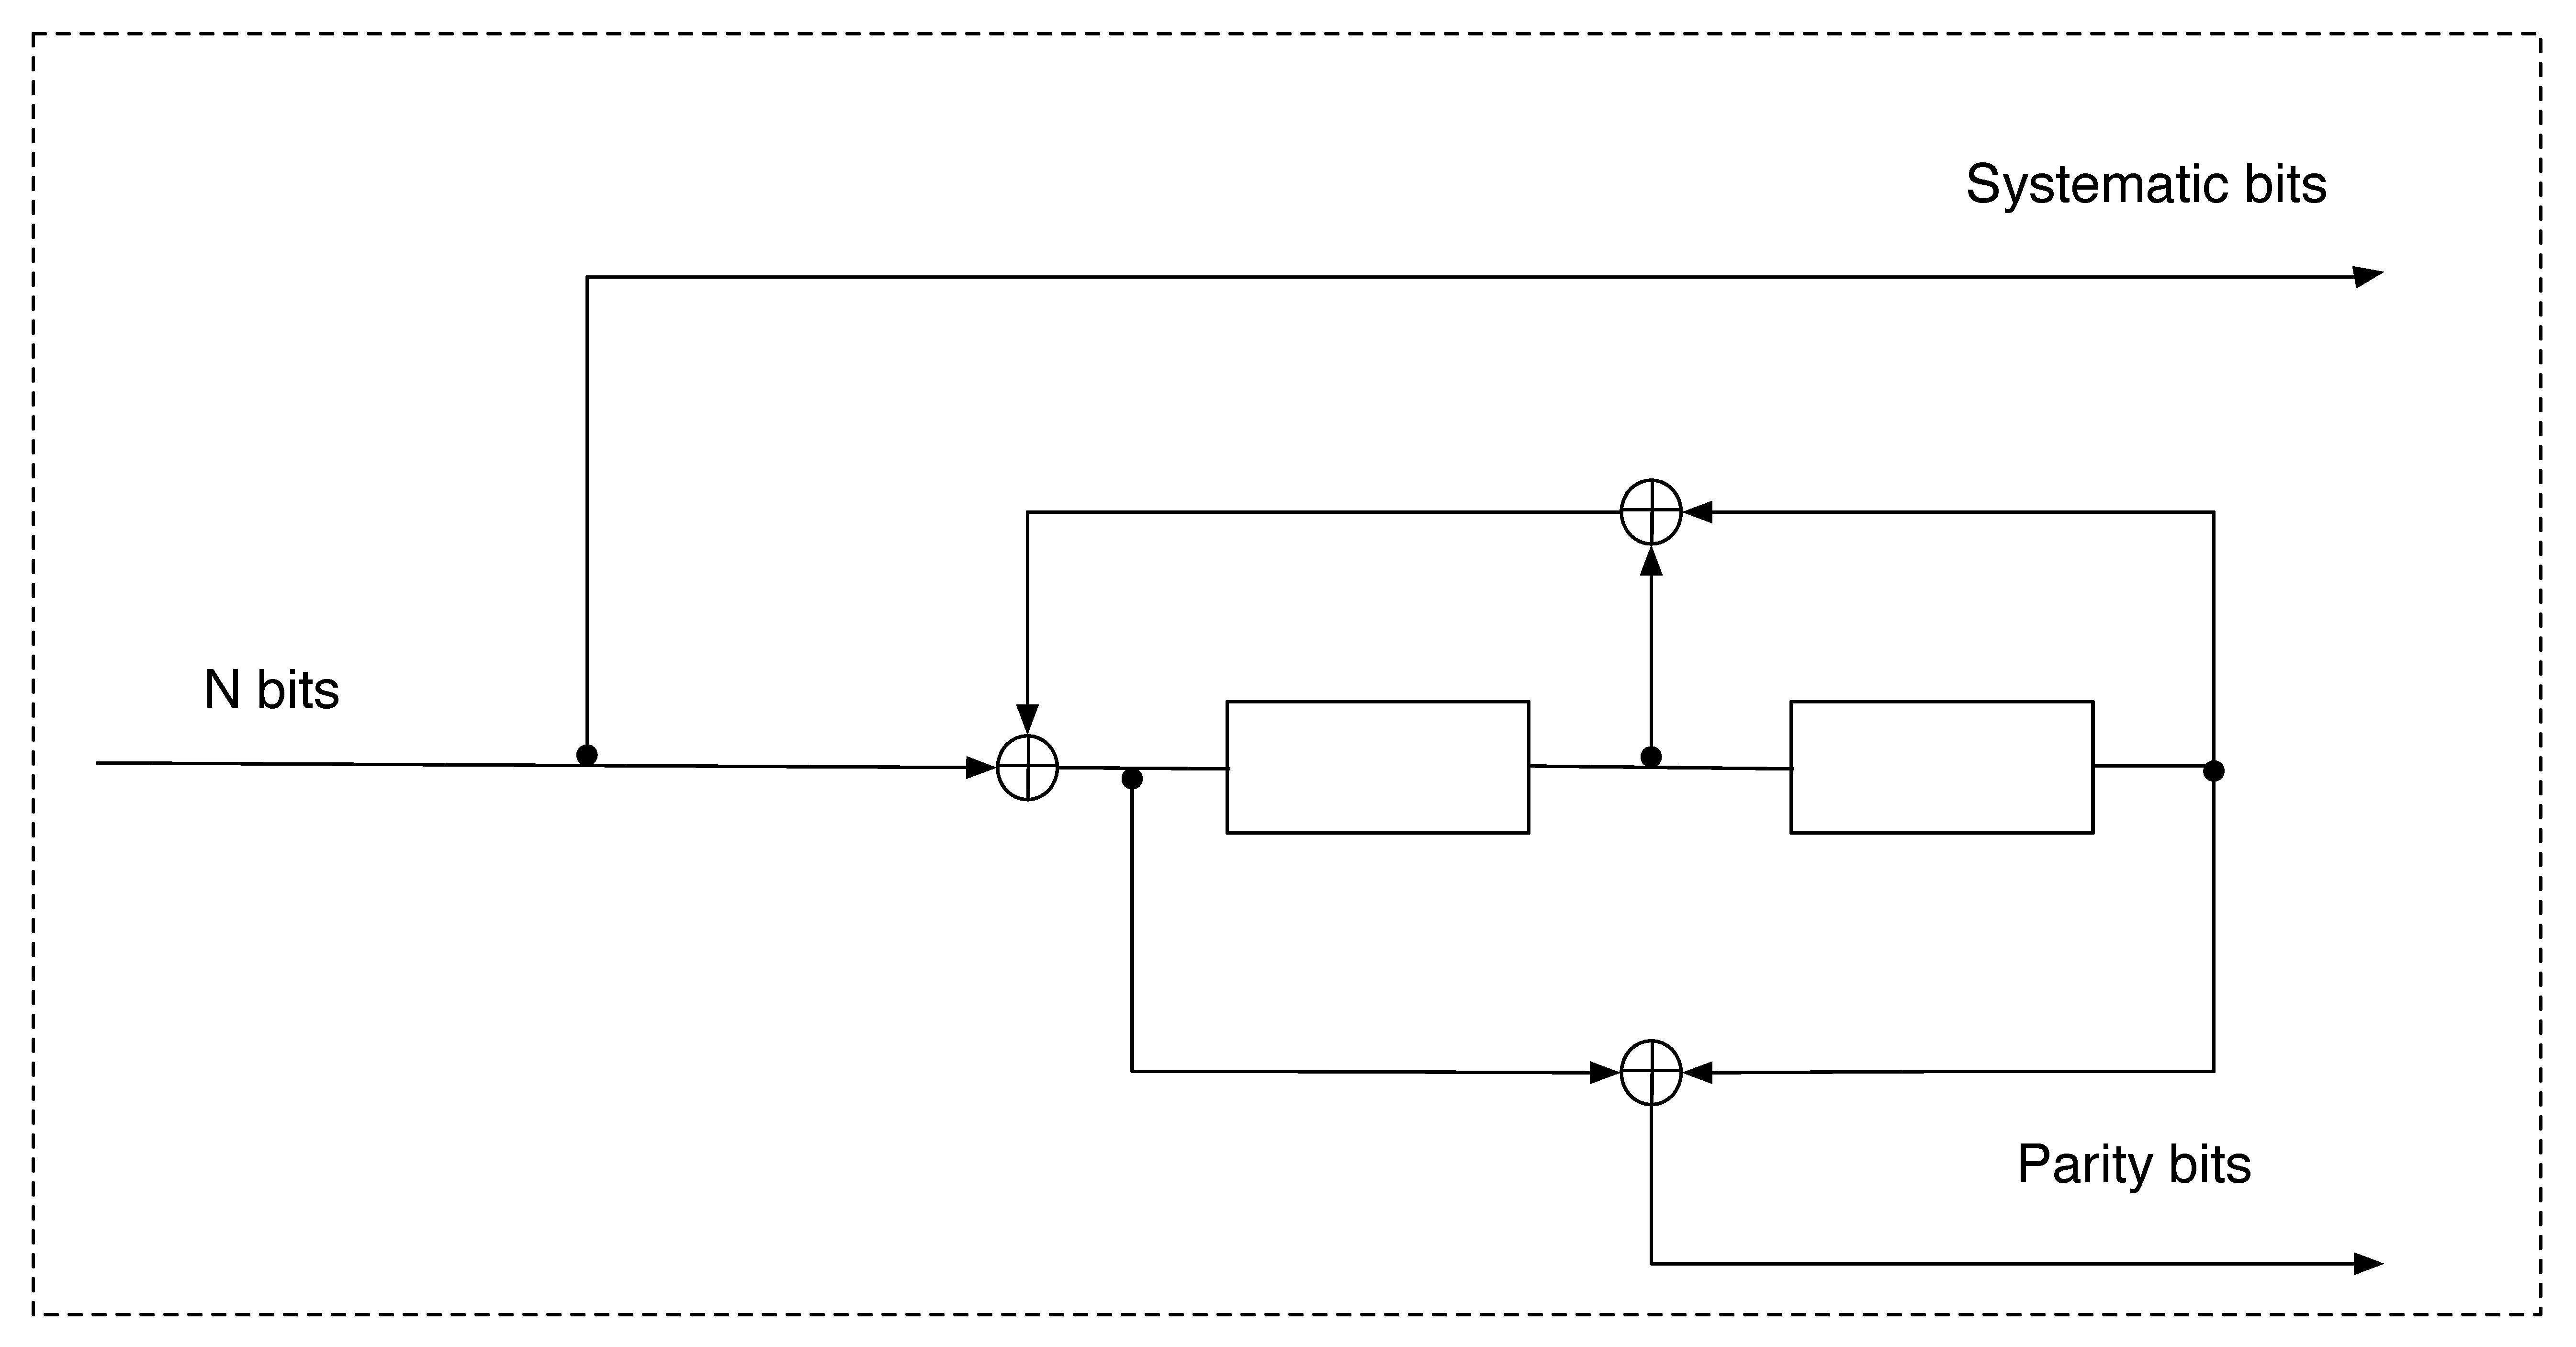
\includegraphics[width=0.45\textwidth]{./PaperSources/RSCExample3.pdf}
	%	\caption{$[\frac{1+x^2}{1+x+x^2}]$  RSC Encoder}
		%\label{fig1}
		%\end{figure}

%\begin{example}		
%An RSC encoder is shown in Figure \ref{fig1} with $k=1$ and $n=2$. Its parity generator\newline function is given by $[\frac{1+x^2}{1+x+x^2}]$, which may be written as $5/7$ in octal form, where $5 ~ \text{and} ~ 7$ correspond to the numerator and denominator of the generator function, respectively. 
 %For this RSC code, the cycle is $\bphi_g=\bphi_6 $ with a cycle length $\tau =3$. While $\bphi=(1~1~1~ 0~ 1~ 1~ 0~ 1~ 1~ 0~\cdots)$, which may be written in terms of the elements of GF(8) as $\bphi_7~\dot{\bphi_3}$ represents the impulse response. 
 %\end{example}
 % Moving forward all other examples and discussions relating to RSC codes will be done using the $5/7$ RSC code unless otherwise stated.

 %The knowledge of $\textbf{p}$ and $\tau$ will be used in deriving the method for determing which input messages generate low-weight parity bits. 